\documentclass[aspectratio=169, 12pt]{beamer}

% Theme
\usetheme{metropolis}
\usepackage{booktabs}
\usepackage{colortbl}
\usepackage{xcolor}
\usepackage{graphicx}
\usepackage{tikz}
\usetikzlibrary{shapes.geometric, arrows.meta, positioning}
\usepackage{pgfplots}
\pgfplotsset{compat=1.18}
\usepackage{multirow}
\usepackage{array}

% ── Global spacing tightening ────────────────────────────────
\setlength{\parskip}{2pt}
\setbeamersize{text margin left=0.7cm, text margin right=0.7cm}
\setbeamertemplate{itemize/enumerate body begin}{\setlength\itemsep{2pt}\setlength\topsep{2pt}}
\setbeamertemplate{itemize/enumerate subbody begin}{\setlength\itemsep{1pt}}

% Colors
\definecolor{ulblue}{RGB}{0, 83, 154}
\definecolor{okgreen}{RGB}{0, 150, 80}
\definecolor{warnred}{RGB}{200, 40, 40}
\definecolor{warnorange}{RGB}{220, 120, 0}
\definecolor{lightgray}{RGB}{240, 240, 240}

\setbeamercolor{frametitle}{bg=ulblue, fg=white}
\setbeamercolor{progress bar}{fg=ulblue}
\setbeamercolor{alerted text}{fg=warnred}

% Macros
\newcommand{\good}[1]{\textcolor{okgreen}{\textbf{#1}}}
\newcommand{\bad}[1]{\textcolor{warnred}{\textbf{#1}}}
\newcommand{\warn}[1]{\textcolor{warnorange}{\textbf{#1}}}

% Metadata
\title{Deep Learning for Content Moderation\\on the Shareish Solidarity Platform}
\subtitle{Progress Report --- Follow-up to April 13, 2026}
\author{Seyfullah Ural\\[4pt]\small Supervisor: Raphaël Marée}
\institute{University of Liège}
\date{May 2026}

% ─────────────────────────────────────────────────────────────
\begin{document}

\maketitle

% ─── BRIDGE: April 13 → May 5 ────────────────────────────────
\begin{frame}[shrink=25]{Since April 13 --- What Changed}
  \textit{\textcolor{gray}{This deck covers work completed between April 13 and May 5, 2026. It assumes
  familiarity with Phase 1 and the two-tier architecture. Thesis chapter drafts are attached separately.}}\\[6pt]
  \small
  \begin{tabular}{p{0.42\textwidth} p{0.02\textwidth} p{0.46\textwidth}}
    \textbf{April 13, 2026 --- Open question} & & \textbf{May 5, 2026 --- Status} \\
    \midrule
    Phase 2 --- LoRA fine-tuning: Reddit-FR adapter pending; joint training hypothesised
    & &
    \good{Complete.} All adapters evaluated; SG-2b $\times$ Reddit-FR LoRA is best (F1 0.662) \\[6pt]

    Phase 3 --- Data collection: planned but not started
    & &
    \warn{In progress.} Track A (1,500 synthetic items) done; Track B scrapers partially running \\[6pt]

    Phase 4 --- Two-tier architecture: design proposed
    & &
    \warn{Under evaluation.} Group 2 done; Tier 1 variant 2c selected; success criterion not yet met \\[6pt]

    Thesis writing --- Early chapter drafts
    & &
    \warn{Advancing.} 1,317 lines across all chapters; Chs 2, 3, 5 most active \\
  \end{tabular}
\end{frame}

% ─── SLIDE 2: Phase 2 Complete ───────────────────────────────
\begin{frame}[shrink=30]{Phase 2 --- LoRA Fine-Tuning: Complete}
  \textit{\small\textcolor{gray}{April 13: Reddit-FR adapter still pending; SG-2b SLURM timeout; joint training
  hypothesised. All resolved.}}\\[4pt]

  \scriptsize
  \begin{tabular}{lcccccc}
    \toprule
    \textbf{Model $\times$ Dataset} & \textbf{Baseline F1} & \textbf{LoRA F1} &
    \textbf{$\Delta$F1} & \textbf{$\Delta$TPR} & \textbf{$\Delta$TNR} & \textbf{Character} \\
    \midrule
    SG-2b $\times$ Reddit-FR & 0.335 & \good{0.662} & \good{+0.327} & +0.415 & $-$0.177 & Recall-driven \\
    LG-1B $\times$ FHS        & 0.371 & \good{0.557} & \good{+0.186} & $-$0.039 & +0.324  & Precision-driven \\
    SG-2b $\times$ FHS        & 0.413 & \good{0.534} & \good{+0.121} & $-$0.007 & +0.149  & Precision-driven \\
    \bottomrule
  \end{tabular}

  \vspace{4pt}
  \small
  FHS adapters are precision-driven (TNR $\uparrow$, models learn what is \emph{not} harmful);
  Reddit-FR adapter is recall-driven (TPR $\uparrow$).
  This distinction guides Tier 2 selection.

  \vspace{4pt}
  \begin{block}{}
    SG-2b $\times$ Reddit-FR LoRA selected as Tier 2 --- best overall F1 (0.662);
    recall substantially improved (+0.415 TPR).
  \end{block}
\end{frame}

% ─── SLIDE 3: Phase 3 Data ───────────────────────────────────
\begin{frame}[shrink=25]{Phase 3 --- Data Collection: Where We Stand}
  \begin{columns}[T]
    \column{0.48\textwidth}
      \textbf{Track A --- Synthetic data \good{(complete)}}\\[3pt]
      \small
      Generated via Mistral-7B-Instruct; HateCheck-FR functionalities:
      slurs, leet-speak, character deletion, implicit derogation, counter-speech.
      \begin{itemize}
        \item 1,500 synthetic items; \good{complete}
        \item Already used in Phase 4 Group 2 (variant 2c)
        \item Note: list-prefix artifact (\texttt{"1. "}) stripped before training
      \end{itemize}

    \column{0.48\textwidth}
      \textbf{Track B --- Scrapers}\\[3pt]
      \scriptsize
      \begin{tabular}{llllp{0.26\linewidth}}
        \toprule
        \textbf{Source} & \textbf{Class} & \textbf{Target} & \textbf{Coll.} & \textbf{Status} \\
        \midrule
        \rowcolor{lightgray}
        donnons.org & solidarity & 3,400 & \good{3,238} & \good{Done} \\
        donnerie.be & solidarity & 1,000 & 0 & \warn{Rerunning (href bug fixed)} \\
        2ememain.be & commercial & 800 & \bad{51} & \bad{Scraper fix needed} \\
        Shareish & solidarity & TBD & TBD & Awaiting supervisor access \\
        \bottomrule
      \end{tabular}
  \end{columns}

  \vspace{4pt}
  \small
  Track B will train a content-type classifier (solidarity\_exchange vs commercial\_listing).
  No classifier trained yet --- awaiting donnerie.be and 2ememain.be.

  \vspace{3pt}
  \begin{alertblock}{Action Item}
    Shareish listing data: access or a sample is needed to complete Track B.
  \end{alertblock}
\end{frame}

% ─── SLIDE 4: Phase 4 Architecture ───────────────────────────
\begin{frame}[shrink=30]{Phase 4 --- Two-Tier Architecture: Current Configuration}
  \begin{columns}[T]
    \column{0.48\textwidth}
      \scalebox{0.78}{%
      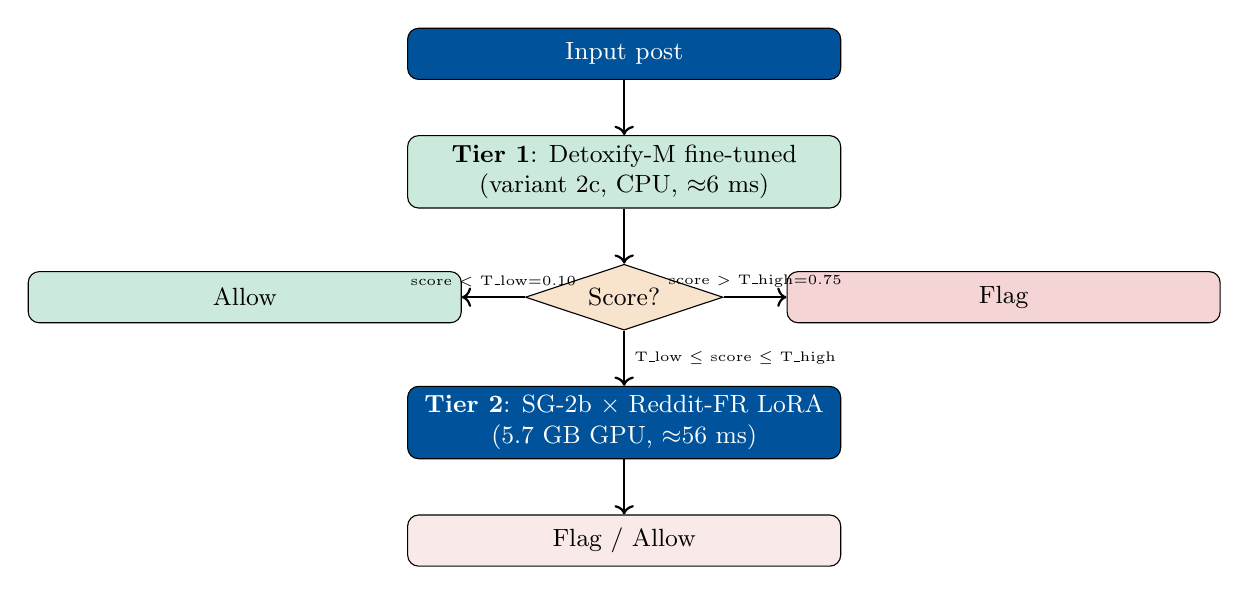
\begin{tikzpicture}[
        node distance=0.7cm,
        box/.style={draw, rounded corners, minimum width=5.5cm, minimum height=0.65cm,
                    font=\small, align=center},
        decision/.style={draw, diamond, fill=warnorange!20, font=\small, align=center, aspect=3},
        arrow/.style={->, thick}
      ]
        \node[box, fill=ulblue, text=white] (input) {Input post};
        \node[box, below=of input, fill=okgreen!20]
              (tier1) {\textbf{Tier 1}: Detoxify-M fine-tuned\\(variant 2c, CPU, $\approx$6 ms)};
        \node[decision, below=of tier1] (dec) {Score?};
        \node[box, left=0.8cm of dec, fill=okgreen!20] (allow) {Allow};
        \node[box, right=0.8cm of dec, fill=warnred!20] (flag1) {Flag};
        \node[box, below=of dec, fill=ulblue, text=white]
              (tier2) {\textbf{Tier 2}: SG-2b $\times$ Reddit-FR LoRA\\(5.7 GB GPU, $\approx$56 ms)};
        \node[box, below=of tier2, fill=warnred!10] (flagallow) {Flag / Allow};
        \draw[arrow] (input) -- (tier1);
        \draw[arrow] (tier1) -- (dec);
        \draw[arrow] (dec) -- node[above, font=\tiny]{score $<$ T\_low=0.10} (allow);
        \draw[arrow] (dec) -- node[above, font=\tiny]{score $>$ T\_high=0.75} (flag1);
        \draw[arrow] (dec) -- node[right, font=\tiny]{T\_low $\leq$ score $\leq$ T\_high} (tier2);
        \draw[arrow] (tier2) -- (flagallow);
      \end{tikzpicture}%
      }

    \column{0.48\textwidth}
      \small\textbf{Key numbers:}
      \begin{itemize}
        \item Tier 1 (variant 2c): Reddit-FR F1 = 0.668, HC-FR F1 = 0.816, FNR = 25.2\%
        \item Tier 2 alone: F1 = 0.640 (511-sample honest holdout)
        \item Combined (75.5\% deferral): F1 = 0.643, avg 47.7 ms
        \item Speed at 10\% deferral: 12.6 ms ($4\times$ faster than Tier 2 alone)
      \end{itemize}

      \vspace{4pt}
      \begin{alertblock}{Success Criterion}
        \small
        Combined F1 $>$ 0.640 at $<$ 30\% deferral ---
        \bad{NOT YET MET}
      \end{alertblock}
  \end{columns}
\end{frame}

% ─── SLIDE 5: Phase 4 Group 2 Tier 1 ────────────────────────
\begin{frame}[shrink=25]{Phase 4 --- Tier 1 Fine-Tuning: Group 2 Results}
  \small
  Four Tier 1 variants evaluated on honest 511-sample holdout (no contamination from
  earlier Tier 1 training runs).\\[4pt]

  \scriptsize
  \begin{tabular}{lcccp{0.36\textwidth}}
    \toprule
    \textbf{Variant} & \textbf{Reddit-FR F1} & \textbf{HC-FR F1} & \textbf{T1\_FNR} & \textbf{Notes} \\
    \midrule
    Track B baseline (3 ep)
      & 0.662 & --- & 41.7\%
      & Bimodal score collapse; data leakage detected \\[3pt]
    2a --- 10 epochs
      & 0.615 & --- & 28.5\%
      & Overfits after epoch 3; no net gain \\[3pt]
    2b --- soft labels ($\varepsilon$=0.05)
      & 0.619 & --- & 28.3\%
      & T1\_FPR: 23.8\%$\to$13.5\% \\[3pt]
    \rowcolor{lightgray}
    \good{2c --- synthetic data (ep 2)}
      & \good{0.668} & \good{0.816} & \good{25.2\%}
      & \good{Best: T\_high breaks to 0.80} \\
    \bottomrule
  \end{tabular}

  \vspace{4pt}
  \small
  Variant 2c selected as Tier 1 for Group 3. Best checkpoint is epoch 2 --- all
  subsequent runs use \texttt{-{}-epochs 2}.

  \vspace{4pt}
  \begin{block}{Group 3 Hypothesis}
    Specialising Tier 2 on the deferred distribution from variant 2c should reduce
    combined-system FNR and push end-to-end F1 above the success threshold at $<$30\% deferral.
  \end{block}
\end{frame}

% ─── SLIDE 6: Phase 4 Speed vs F1 ────────────────────────────
\begin{frame}[shrink=30]{Phase 4 --- End-to-End: Speed vs.\ F1 Trade-off}
  \begin{columns}[T]
    \column{0.52\textwidth}
      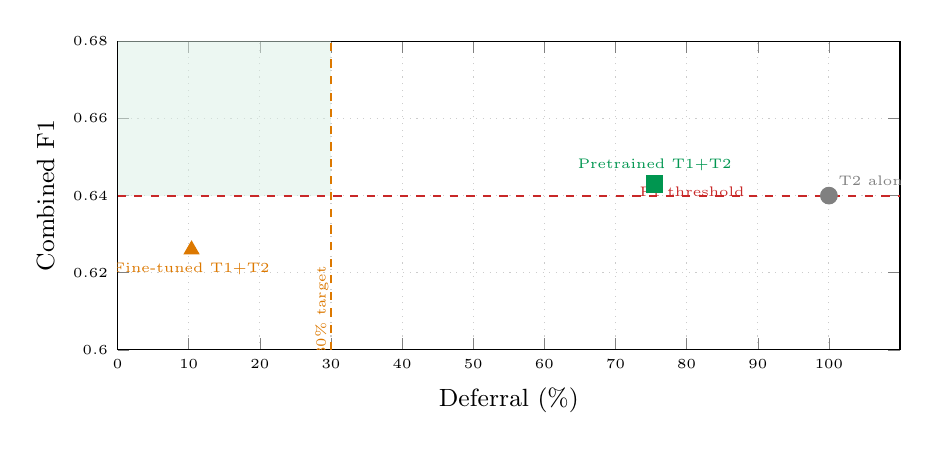
\begin{tikzpicture}
        \begin{axis}[
          width=0.95\linewidth, height=5.5cm,
          xlabel={Deferral (\%)}, ylabel={Combined F1},
          xmin=0, xmax=110, ymin=0.60, ymax=0.68,
          xtick={0,10,20,30,40,50,60,70,80,90,100},
          ytick={0.60,0.62,0.64,0.66,0.68},
          grid=major, grid style={dotted,gray!40},
          legend pos=south east, legend style={font=\tiny},
          tick label style={font=\tiny}, label style={font=\small},
        ]
          % Success zone shading (F1 > 0.640 AND deferral < 30%)
          \addplot[fill=okgreen!15, draw=none, opacity=0.5]
            coordinates {(0,0.640)(30,0.640)(30,0.68)(0,0.68)} -- cycle;
          % F1 success threshold
          \addplot[dashed, color=warnred, thick]
            coordinates {(0,0.640)(110,0.640)};
          \node[font=\tiny, color=warnred, anchor=west]
            at (axis cs:72,0.641) {F1 threshold};
          % Deferral target
          \addplot[dashed, color=warnorange, thick]
            coordinates {(30,0.60)(30,0.68)};
          \node[font=\tiny, color=warnorange, anchor=south, rotate=90]
            at (axis cs:31,0.61) {30\% target};
          % Data points
          \addplot[only marks, mark=*, mark size=3pt, color=gray]
            coordinates {(100,0.640)};
          \node[font=\tiny, color=gray, anchor=south west]
            at (axis cs:100,0.640) {T2 alone};
          \addplot[only marks, mark=square*, mark size=3pt, color=okgreen]
            coordinates {(75.5,0.643)};
          \node[font=\tiny, color=okgreen, anchor=south]
            at (axis cs:75.5,0.644) {Pretrained T1+T2};
          \addplot[only marks, mark=triangle*, mark size=3pt, color=warnorange]
            coordinates {(10.4,0.626)};
          \node[font=\tiny, color=warnorange, anchor=north]
            at (axis cs:10.4,0.625) {Fine-tuned T1+T2};
        \end{axis}
      \end{tikzpicture}

    \column{0.44\textwidth}
      \scriptsize
      \begin{tabular}{lccc}
        \toprule
        \textbf{Config} & \textbf{F1} & \textbf{Deferral} & \textbf{Avg ms} \\
        \midrule
        T2 alone          & 0.640        & 100\%              & 55.9 \\
        Pretrained T1+T2  & \good{0.643} & 75.5\%             & 47.7 \\
        Fine-tuned T1+T2  & 0.626        & \good{10.4\%}      & \good{12.6} \\
        \bottomrule
      \end{tabular}

      \vspace{6pt}
      \small\textit{Speed advantage is real ($4\times$ at low deferral), but no configuration
      simultaneously achieves F1 $>$ 0.640 AND deferral $<$ 30\%. Group 3 targets this gap.}
  \end{columns}
\end{frame}

% ─── SLIDE 7: Remaining Work ─────────────────────────────────
\begin{frame}[shrink=20]{Remaining Work --- Phases 3 \& 4}
  \begin{columns}[T]
    \column{0.48\textwidth}
      \textbf{Phase 3 --- remaining:}
      \begin{itemize}
        \item Rerun donnerie.be scraper (href bug fixed); target 1,000 items
        \item Fix 2ememain.be Dutch-language filter; target 800 items
        \item Train content-type classifier once Track B complete
        \item Evaluate classifier on Shareish listing sample
      \end{itemize}

    \column{0.48\textwidth}
      \textbf{Phase 4 --- remaining:}
      \begin{itemize}
        \item Simulate end-to-end with variant 2c + SG-2b LoRA on 511-sample holdout
        \item Group 3: Tier 2 specialisation on deferred distribution at T=(0.10, 0.75)
        \item Stretch: SG-2b retrain (LR=$10^{-4}$, balanced joint adapter 1:1 FHS:Reddit-FR)
      \end{itemize}
  \end{columns}

  \vspace{8pt}
  \begin{block}{Definition of Done}
    Architecture complete when: combined F1 $>$ 0.640 AND deferral $<$ 30\%.
  \end{block}
\end{frame}

% ─── SLIDE 8: Thesis Writing ─────────────────────────────────
\begin{frame}[shrink=20]{Thesis Writing --- Current Status}
  \small
  \begin{tabular}{llcc}
    \toprule
    \textbf{Chapter} & \textbf{Topic} & \textbf{Lines} & \textbf{Status} \\
    \midrule
    Introduction & Motivation, Shareish, research plan & 76 & \warn{Draft} \\
    Ch 1 --- Background & NLP, hate speech, content moderation & 193 & \warn{Draft} \\
    Ch 2 --- Framework & Models, datasets, metrics & 227 & In progress \\
    Ch 3 --- Phase 1 Results & Baseline evaluation & 351 & In progress \\
    \cellcolor{warnred!15}Ch 4 --- Data Strategy & \cellcolor{warnred!15}Scraping + synthetic generation & \cellcolor{warnred!15}71 & \cellcolor{warnred!15}\bad{Stub} \\
    Ch 5 --- LoRA Fine-tuning & Phase 2 results & 184 & In progress \\
    Ch 6 --- Conclusions & Architecture recommendation & 117 & \warn{Draft} \\
    \midrule
    \rowcolor{lightgray}
    \textbf{Total} & & \textbf{1,317} & --- \\
    \bottomrule
  \end{tabular}

  \vspace{4pt}
  \small
  Chapters 3 and 5 are most advanced, reflecting completed experimental phases.
  Chapter 4 will expand once Phase 3 data results are available.

  \vspace{4pt}
  \begin{alertblock}{}
    Attached to this email: [list chapters].
    \textbf{Feedback most welcome on:} [priority sections].
  \end{alertblock}
\end{frame}

% ─── SLIDE 9: Questions ──────────────────────────────────────
\begin{frame}[shrink=15]{Questions \& Feedback Sought}
  \begin{enumerate}
    \setlength\itemsep{8pt}
    \item \textbf{Phase 4 success criterion} --- The current target (F1 $>$ 0.640 at
          $<$ 30\% deferral) was self-defined. Is this the right criterion, or should it
          be reframed (e.g.\ FNR $<$ 25\%, or a latency target alone)?

    \item \textbf{Group 3 scope} --- Given the combined F1 gap is only 0.014, is
          Tier 2 specialisation worth the remaining SLURM time, or should effort shift
          to writing?

    \item \textbf{Content-type classifier (Track B)} --- Is this a thesis-depth
          contribution or better placed in an appendix?

    \item \textbf{Chapter 4 --- Data Strategy} is currently a 71-line stub.
          Guidance on expected scope and depth is welcome.

    \item \textbf{Attachments} --- Which of the attached chapter drafts should be
          prioritised for review?
  \end{enumerate}
\end{frame}

\end{document}
